%!TEX spellcheck=ro_RO
%!TEX root = ./main.tex
\chapter{Introducere}\label{ch:1intro}
Ceva despre istoria AI
\section{Temă. Obiective. Motivație}
\textbf{TODO Edit First Paragraph}

Tehnicile de învățare automată urmăresc crearea unor modele matematice bazate pe seturi de date inițiale, denumite \textit{seturi de antrenare (training data)}, care pot generaliza informațiile din acestea, iar mai apoi să prezică răspunsul pentru seturi de date necunoscute.

Învățarea automată este folosită intr-o largă gamă de aplicații, precum filtrarea mesajelor e-mail de tip spam de cele autentice, răspunsurile date de către motoarele de căutare, clasificarea celulelor tumorale in benigne sau maligne, recunoașterea facială, recunoașterea diverselor obiecte, recunoașterea limbajului vorbit și scris, și mai nou la conducerea automată a mașinilor. 

Cele mai multe tehnici de învățare automată fac parte din una dintre cele trei categori:
\begin{itemize}
	\item Învățare supervizată (Supervised Learning)
	\item Învățare nesupervizată (Unsupervised Learning)
	\item Învățare cu întărire (Reinforcement Learning)
\end{itemize}

\subsection*{Învățarea supervizată}
Învățarea supervizată, în momentul de fața este cea mai răspandită metodă folosită în practică. Principiul din spatele acesteia constând în construirea unui model matematic, prin diferite tehnici, bazat pe un set de date etichetate. Acest set de date etichetate este alcătuit din înregistrări care reprezintă o corespondență intre atribute (intrări) si o clasă (ieșire). Astfel, se urmărește generalizarea acestor corespondețe si posibilitatea prezicerii clasei unei înregistrări care nu aparține de datele folosite la învățare. Unii dintre cei mai folosiți algoritmi de învățare supervizată sunt:
\begin{itemize}
	\item Arbori de decizie
	\item Metode de regresie
	\item Algoritmi genetici
	\item Rețele neuronale artificiale
	\item Mașini cu vector suport
	\item Rețele Bayesiene
\end{itemize}

\subsection*{Învățarea nesupervizată}
Procesul de învățare nesupervizată diferă față de cel amintit anterior prin faptul că acesta folosește un set de date de antrenare neetichetat. Algoritmii primesc doar un set de atribute (date de intrare), ne știind ieșirea asociată acestora. Aceștia caută in aceste date asemănări și deosebiri, bazându-se pe proprietățile statistice a datelor. Printre cele mai răspândite tehnici se numără:
\begin{itemize}
	\item Tehnici de grupare
	\subitem Grupare ierarhizată
	\subitem Tehnica k-means
	\item Hărți cu auto-organizare
	\subitem Rețele Kohonen
	\item Modele Markov cu stări invizibile
\end{itemize}
\begin{figure}[h]
	\center
	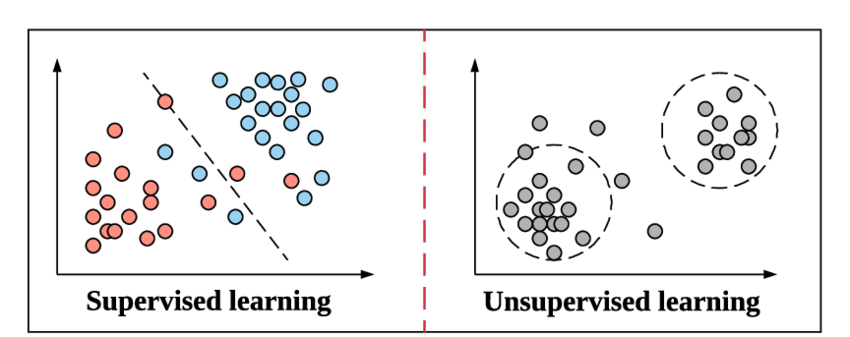
\includegraphics[width=12cm, keepaspectratio]{fig/Examples-of-Supervised-Learning-Linear-Regression-and-Unsupervised-Learning.png}
	\caption{Diferența dintre modul de funcționare al învățării supervizare și învățării nesupervizate \cite{fig:sup_and_unsup}}
	\label{fig:sup_and_unsup_learning}
\end{figure}

\subsection*{Învățarea cu întărire}
Învățarea cu întărire este o metodă de învățare prin interacțiuni repetate a unui \textit{agent (software agent)} cu mediul, cu urmărirea atingerii unui anumit scop (\autoref*{fig:reinf_learning}). Interacțiunile se bazează pe acțiunile luate de agent la stimulii mediului, pentru care v-a primit o recompensă de la acesta în funcție de beneficiul adus îndeplinirii scopului. Recompensele primite au rolul de a îmbunătății capacitatea agentului de a lua cea mai bună decizie din starea în care acesta se afla la momentul acțiunii. Scopul pe termen lung al agentului este maximizarea numărului de recompense primite. După repetate interacțiuni cu mediul, capacitatea agentului de a lua decizii bune se v-a crește, iar drumul acestuia prin mediu va tinde spre optim.
\begin{figure}[h]
	\center
	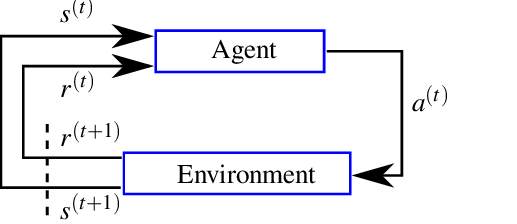
\includegraphics[width=11cm, keepaspectratio]{fig/The-reinforcement-learning-paradigm-consists-of-an-agent-interacting-with-an.png}
	\caption{Modul de funcționare al învățării cu întărire \cite{fig:reinforcement}}
	\label{fig:reinf_learning}
\end{figure}

\subsection*{Obiective}
Această lucrare își propune folosirea rețelelor convoluționale pentru clasificarea a trei clase/stării mentale diferite. Metoda de clasificare se bazează pe reprezentarea informațiilor statistice și spectrale a undelor cerebrale sub forma unor imagini alb-negru. Datele EEG \textit{(Electroencefalograma)} au fost extrase cu ajutorul caștii valabile comercial, Muse 2016. Datele extrase au fost prelucrate și etichetate, rezultând 414 atribute și clasa de care aparțin, neutru, relaxat sau concentrat. După extragerea atributelor, au fost selectate și normalizate în intervalul [0:1] 400 de atribute pentru a putea reprezenta o imagine alb-negru de dimensiunea 20x20. După antrenarea clasificatorului cu aceste imagini, acuratețea acestuia la prezicerea imaginilor care nu se aflau in setul de date de antrenare, a fost de 90\%.

\section{Soluții existente}
Apariția unor soluții comerciale \textit{low-cost} non-invazive a facut posibilă înregistrarea și analiza undele cerebrale în afara domeniului medical \cite{online:emotiv}. Cu toate că acestea sunt folosite în principal în activități simple de interfațare a creerului cu calculatorul \textit{(BCI - Brain-Computer Interface)}, apar tot mai multe studii științifice care folosesc aceste aparate.

EEG-CNN\cite{EEG-CNN:2020}



EEG\cite{EEG:2018}

\textbf{TODO\_PLACEHOLDER}
\begin{itemize}
	\item Utilizare casca pt clasificare EEG de detectare a starii
	\subitem Scriu despre articolul de clasificare EEG de la cei care au scris articolul cu CNN
	\subitem O sa scriu despre articolul cu CNN
	\subitem O sa mai caut niste detalii
\end{itemize}
\section{Structurare pe capitole}